\chapter{Estado del arte}\label{cap:estado}

\section{Contextualización}

La planificación temporal y académica son pilares indispensables para un buen desempeño en el entorno universitario. Para los alumnos de centros con una estructura académica compleja, o profesores con varias horas de docencia en diferentes grupos, como la Escuela Técnica Superior de Ingenierías Informática y de Telecomunicación (ETSIIT) de la Universidad de Granada (UGR), la capacidad de organizar y visualizar sus horarios de manera clara y personalizada se convierte en una necesidad notable.
\newline\newline
La gestión de múltiples asignaturas, grupos de teoría y prácticas, seminarios, tutorías y actividades personales requiere de herramientas que vayan más allá de la simple presentación estática de información, y además de manera general para toda la institución.
\newline\newline
Sin embargo, los sistemas tradicionales de visualización de horarios en muchas instituciones académicas presentan limitaciones significativas. De manera frecuente, la información se ofrece en formatos estáticos, como documentos PDF o imágenes, que dificultan la personalización, la interacción, la integración con las herramientas digitales que los estudiantes utilizan en su día a día, y en algunos casos una visibilidad accesible.
\newline\newline
Esta falta de dinamismo y personalización puede generar confusión, dificultar la planificación y no aprovechar las ventajas que ofrecen las tecnologías actuales para una gestión académica más eficiente y adaptada a las necesidades individuales.
\newline\newline
Este capítulo presenta una revisión del estado del arte que fundamenta la necesidad y el enfoque del proyecto. Se analiza la situación actual de la gestión y visualización de horarios en la UGR. 
Posteriormente, se realizará un análisis comparativo con sistemas más avanzados implementados en otras instituciones de educación superior. A continuación, se profundizará en los paradigmas arquitectónicos de backend, justificando la elección de una arquitectura de microservicios frente a un enfoque monolítico tradicional. Finalmente, se examinará y justificará la selección del stack tecnológico propuesto, incluyendo Java y el ecosistema Spring para el desarrollo de microservicios, RabbitMQ para la comunicación asíncrona, la combinación de bases de datos MySQL y MongoDB bajo el principio de persistencia políglota, la librería Jsoup para la adquisición de datos mediante web scraping, y las tecnologías empleadas para el despliegue del sistema, como Docker.

\section{Visualización y gestión de horarios académicos en la UGR}

La Universidad de Granada, al igual que muchas otras universidades descentraliza sus sedes, de modo que
cada una de ellas tiene su propio sistema de gestión de la información. En este sentido, las facultades cuentan
con una serie de sistemas de información propios que se encargan de la generación de horarios académicos,
asignación de aulas y profesores a los grupos tanto de teoría como de prácticas 
de las distintas titulaciones y asignaturas.sta información a su vez se le facilita a la Universidad de Granada para la centralización de la información.
\newline\newline
Para acceder a la información de los horarios, los estudiantes y docentes pueden hacerlo de diferentes maneras:
\begin{itemize}
    \item A través de la página propia de su facultad. Poniéndo de ejemplo a la ETSIIT, debemos acceder a la página oficial de la facultad \cite{webETSIIT} y buscar la información en la sección
          de ``Calendario de exámenes`` en caso de querer saber los días y rangos horarios de estos y visualizándolo con un pdf, o a ``Calendario académico y horarios`` y a ``Grado en Ingeniería Informática``
          en caso de querer saber los horarios de los diferentes grupos del grado, presentado todo ello en un pdf contenedor de alrededor de 40 tablas.
          \newline\newline
          De esta manera tendremos que buscar el año al que pertenece la asignatura de la que estamos matriculados y el grupo al que pertenecemos. De esta manera obtenemos su 
          franja horaria y aula, pero no profesor que imparte la asignatura.
          \newline\newline
          Sin embargo, el formato de las tablas cambia de un grado a otro, haciendo que el estudiante tenga que buscar la información de manera diferente en cada grado si está matriculado en más de uno, 
          y obteniendo información diferente. En el caso del grado de Administración y Dirección de Empresas por ejemplo, no se muestra el aula en la que se imparte la clase, pero sí las asignaturas bilingües, y
          los profesores que las imparten.
          \newline\newline
          Esta forma de visualización de horarios es muy poco eficiente, ya que el estudiante tiene que buscar la información de manera manual, es inconsistente entre grados, y no es accesible para personas con discapacidad visual.
          %% Comparación de horarios de diferentes grados ( 2 imágenes )
          %% Como se insertan dos imagenes en latex con un unico pie de foto -> 
          \newpage
            \begin{figure}[H]
                \centering
                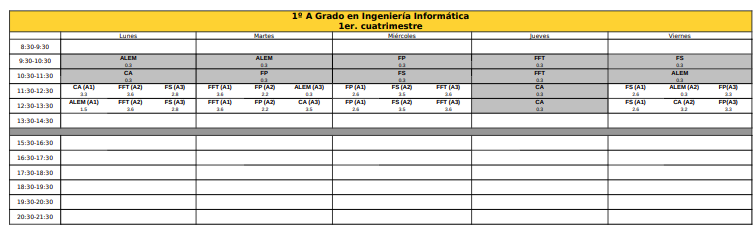
\includegraphics[width=0.8\textwidth]{figures/02_etsiit_horario.png}
                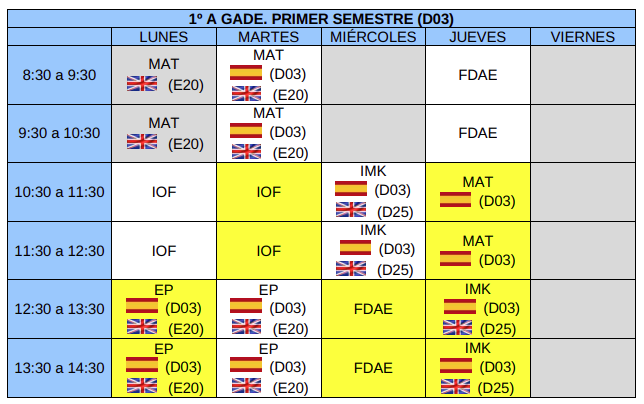
\includegraphics[width=0.8\textwidth]{figures/02_ade_horario.png}
                \caption{Comparación de horarios de diferentes grados: ETSIIT (arriba) y ADE (abajo).}
                \label{fig:horarios_comparacion}
            \end{figure}
          

    \item A través de la web grados UGR \cite{webGrados} se puede buscar la información de los horarios de las asignaturas de los diferentes grados de la Universidad de Granada. Para ello debemos seleccionar rama de conocimiento, 
          grado, curso y asignatura. De esta manera obtenemos un horario semanal con las franjas horarias, aulas, profesores y fechas tanto de inicio como de fin. Este método nos proporcioan una interfaz estándar y más información, pero 
          también es más lento y tedioso para consultar por varias asignaturas o incluso grados.
    \item A través de las webs de cada departamento. Por ejemplo en la web del departamento de Ciencias de la Computación e Inteligencia Artificial \cite{webDecsai} se puede consultar la información de las asignaturas o profesores de este.
          Ofrece información adicional como asignaturas que imparte ``x'' profesor y su horario de tutorías y docencia.
\end{itemize}

Además para acceder a la información de periodos de actividad docente, exámenes finales, periodos de evaluación de convocatorias ... se ha de acceder a la web de la Secretaría General en la UGR \cite{webSecretaria} para consultar otro pdf.

En general la información de los horarios académicos de la Universidad de Granada es poco accesible, eficiente y consistente entre grados y facultades, lo que hace que el estudiante tenga que buscar la información de manera manual y tediosa.
Además no hay manera de consultar de manera sencilla un calendario personal que incluya tanto los horarios de las asignaturas como los exámenes y periodos de evaluación, entre otros.
\newline\newline
Pongamos el ejemplo de un estudiante matriculado en el primer curso del Grado de Biología en la Universidad de Granada con el estándar de cinco asignaturas en su primer cuatrimestre. 
Este estudiante tiene que buscar la información de los horarios de las asignaturas en la web de su facultad, en la web de la Universidad de Granada o en la web del departamento al que pertenezca cada asignatura.
Suponemos que decide buscar su horario en la web de grados ugr, y una vez seleccionada la rama de conocimiento, grado, curso y asignatura, obtiene un horario semanal con las franjas horarias de todos los grupos de la asignatura, aulas, profesores y fechas tanto de inicio como de fin.
Está matriculado por ende en la asignatura ''Bases Químicas de la Biología'' en el grupo ``A'' de teoría y en el grupo ``2'' de prácticas, por lo que tiene que buscar los sectores que pertenecen a su grupos para poder obtener su horario personalizado para esa materia.
\newline\newline
La realidad con la que se encuentra el estudiante es con la siguiente:

\begin{figure}[H]
    \centering
    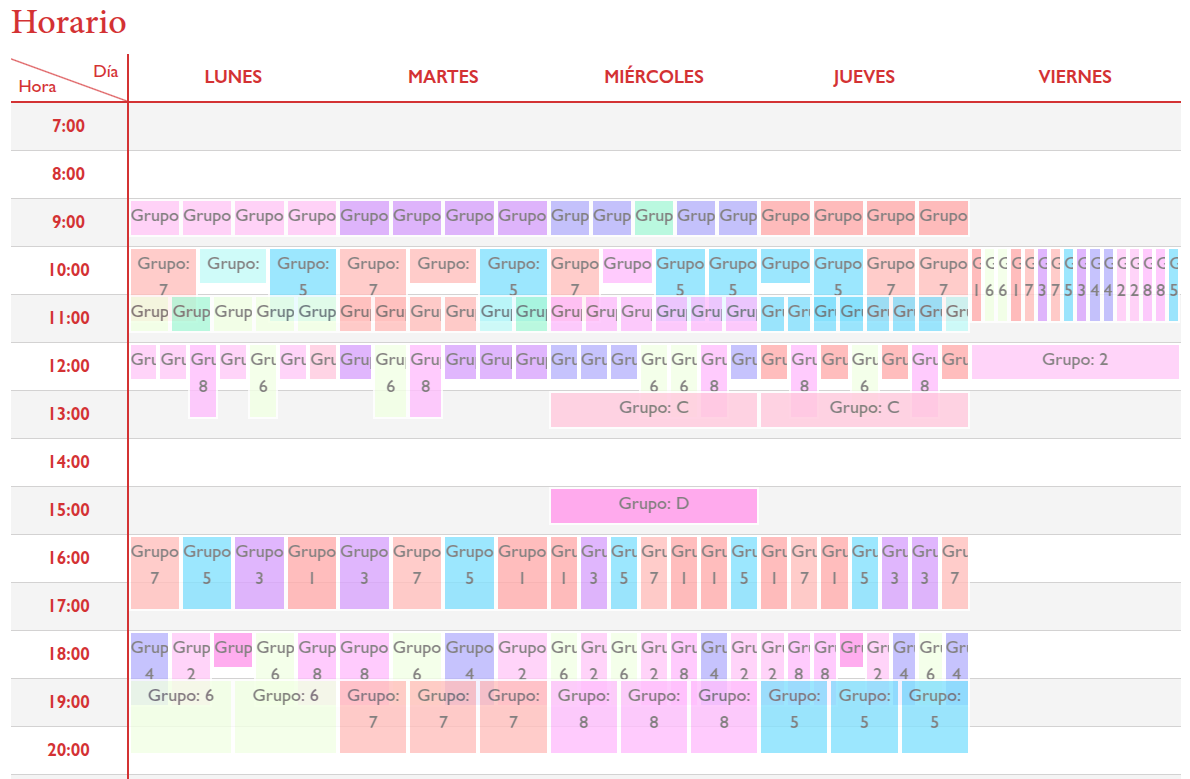
\includegraphics[width=0.8\textwidth]{figures/02_horario_biologia.png}
    \caption{Horario de la asignatura Bases Químicas de la Biología.}
    \label{fig:horario_biologia}
\end{figure}

El estudiante tiene que dedicar un tiempo considerable en buscar las franjas pertenecientes a sus grupos, puesto que no hay una sencilla visualización de los mismos. Además se requiere una búsqueda activa con el cursor
para poder ver las franjas ocultas, y esta acción puede resultar tediosa cuando hay muchos sectores juntos, como en este caso.

Podemos concluir tras analizar la situación actual de aprovisionamiento de horarios académicos a los usuarios de la Universidad de Granada, que surge la necesidad de un sistema que permita la visualización de horarios académicos de manera sencilla, accesible y personalizada.

\section{Análisis comparativo de sistemas de planificación personalizada en educación superior}

Frente al modelo estático observado de manera generalizada en la Universidad de Granada, el panorama de la gestión de horarios en otras instituciones de educación superior y en el mercado de software educativo muestra una clara tendencia hacia sistemas más dinámicos, personalizados e integrados. 
\newline\newline
Existen diversas soluciones, desde módulos dentro de grandes sistemas ERP educativos hasta herramientas especializadas en la creación y gestión de horarios y planificadores académicos \cite{webModernCampus}, pasando por aplicaciones de seguimiento del tiempo adaptadas al ámbito educativo.
El análisis de estas herramientas revela un conjunto de características comunes y avanzadas que definen el estado del arte en este dominio:

\begin{itemize}
      \item 
\end{itemize}
\section{Arquitectura de microservicios}

\section{Conclusión}

